\pdfoutput=1
\documentclass{article} % For LaTeX2e
\usepackage{iclr2017_workshop,times}
\usepackage{hyperref}
\usepackage{url}

% my imports
\usepackage{amssymb,amsmath,amsthm}
\usepackage[makeroom]{cancel}
\usepackage{algorithm}
\usepackage[noend]{algpseudocode}
\usepackage{graphicx}
\usepackage{multirow,bigstrut}
\newcommand{\eqname}[1]{\tag*{#1}}

\usepackage{textcomp}

\title{Reinterpreting Importance-Weighted \\Autoencoders}


\author{Chris Cremer, Quaid Morris \& David Duvenaud \\
Department of Computer Science\\
University of Toronto\\
%Toronto, ON, Canada \\
\texttt{\{ccremer,duvenaud\}@cs.toronto.edu} \\
\texttt{\{quaid.morris\}@utoronto.ca}
% \texttt{ccremer@cs.toronto.edu},\texttt{quaid.morris@utoronto.ca},\texttt{duvenaud@cs.toronto.edu}\\
}

\newcommand{\fix}{\marginpar{FIX}}
\newcommand{\new}{\marginpar{NEW}}

\begin{document}


\maketitle

\begin{abstract}
The standard interpretation of importance-weighted autoencoders is that they maximize a tighter lower bound on the marginal likelihood.
We give an alternate interpretation of this procedure: that it optimizes the standard variational lower bound, but using a more complex distribution. 
We formally derive this result, and visualize the implicit importance-weighted approximate posterior.
%This distribution, $q_{IW}(z|x)$, is an importance weighted distribution implicitly defined by the  a pointwise reweighting of a parametric base distribution $q(z|x)$.
%We also propose a family of extensions allowing iterative refinement of the approximate posterior based on gradients of the log-likelihood.
\end{abstract}
 

\begin{figure}[b]
  \centering
   True posterior \qquad  \qquad $k=1$  \qquad \qquad \qquad $k=10$ \qquad \qquad \qquad $k=100$ \quad
      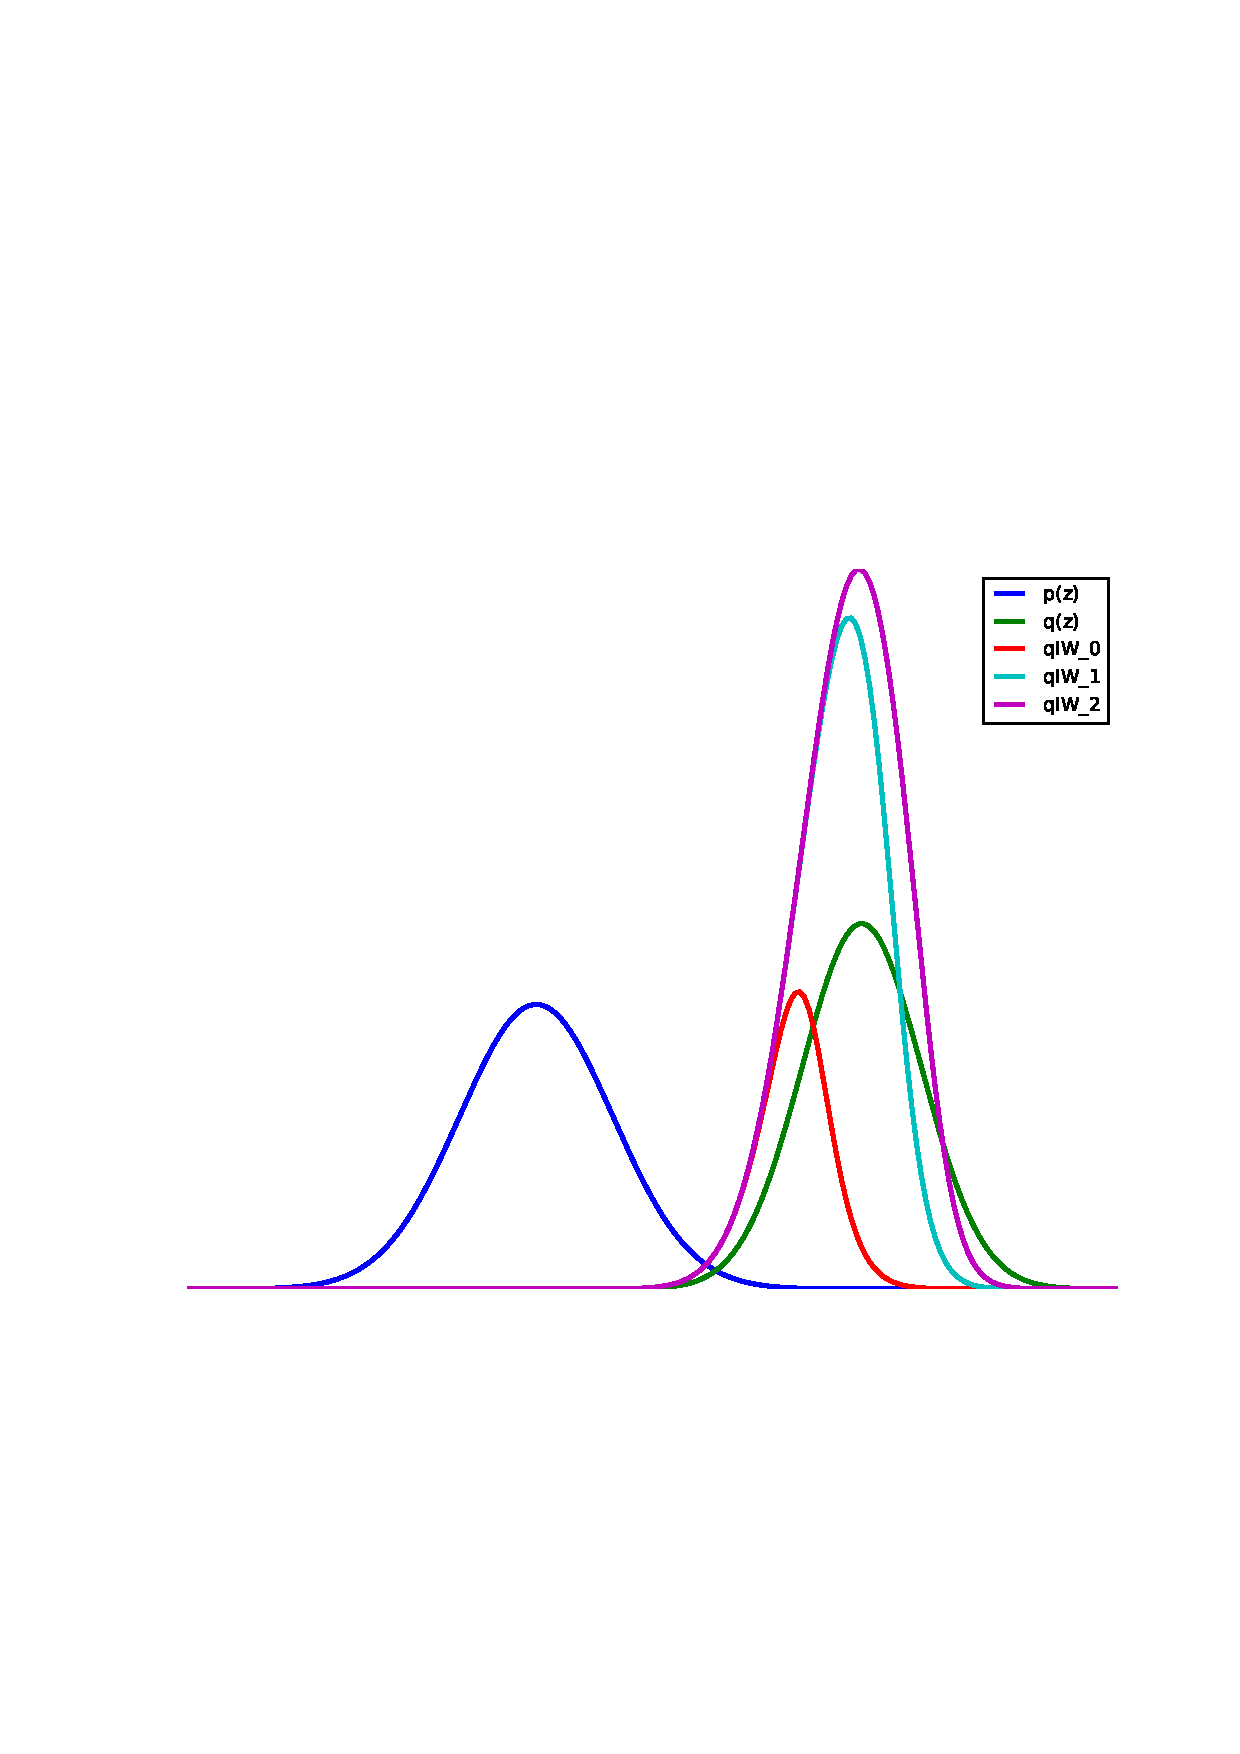
\includegraphics[width=1.\textwidth, clip, trim=2.5cm 3.9cm 2cm 3.6cm]{figs/figure_1.png}
  \vspace{-5mm}
  \caption{Approximations to a complex true distribution, defined via $q_{EIW}$.
%   sampling-importance-resampling. 
  As $k$ grows, this approximation approaches the true distribution.}
  \label{viz1}
\end{figure}


\section{Background}
The importance-weighted autoencoder (IWAE; \cite{burda2015importance}) maximizes the following multi-sample evidence lower bound (ELBO): 
\begin{align} 
    log(p(x)) &
    % log\left(E_{z_{1}...z_{k} \sim q(z|x)} \left[  \frac{1}{k}\sum_{i=1}^k \frac{p(x,z_i)}{q(z_i|x)}    \right]   \right)_{ML}
    % \\
    % & 
    \geq E_{z_{1}...z_{k} \sim q(z|x)} \left[log\left(  \frac{1}{k}  \sum_{i=1}^k \frac{p(x,z_i)}{q(z_i|x)}  \right)  \right] = L_{IWAE}[q] \label{iwae_elbo}  \eqname{(IWAE ELBO)}
\end{align}
which is a tighter lower bound than the ELBO maximized by the variational autoencoder (VAE; \cite{vae}):
\begin{align}
    log(p(x)) & \geq E_{z_{1}...z_{k} \sim q(z|x)} \left[  \frac{1}{k}\sum_{i=1}^k log\left(\frac{p(x,z_i)}{q(z_i|x)}  \right)  \right] = L_{VAE}[q]. \label{vae_elbo} \eqname{(VAE ELBO)}
\end{align}
Here we've written the VAE bound as a multisample lower bound to compare it to the IWAE bound. The following equations are the gradients of the VAE ELBO and the IWAE ELBO, respectively:
\begin{align} 
    \nabla_{\Theta} \mathcal{L}_{VAE}[q] &= E_{z_{1}...z_{k} \sim q(z|x)} \left[   \sum_{i=1}^k \frac{1}{k} \nabla_{\Theta} log\left(\frac{p(x,z_i)}{q(z_i|x)}  \right)  \right] \label{vae_grad} \\
% \end{align}
% \begin{align} 
    \nabla_{\Theta} \mathcal{L}_{IWAE}[q] &= E_{z_{1}...z_{k} \sim q(z|x)} \left[  \sum_{i=1}^k \tilde{w}_i \nabla_{\Theta} log\left(\frac{p(x,z_i)}{q(z_i|x)}  \right)  \right] \label{iwae_grad}
\end{align}
where $$\tilde{w}_i = \frac{\frac{p(x,z_i)}{q(z_i|x)}}{\sum_{j=1}^k \frac{p(x,z_j)}{q(z_j|x)}}.$$

From equations \eqref{vae_grad} and \eqref{iwae_grad}, we see that the gradient of the VAE ELBO evenly weights the samples, whereas the IWAE gradient weights the samples based on their relative importance $\tilde{w}_i$.






\section{Defining the implicit distribution \texorpdfstring{$q_{IW}$}{}}

%From the gradient of the IWAE bound (Eqn. \ref{iwae_grad}), we know that each sample is weighted by their importance $\tilde{w}_i$. This weighting implicitly defines a nonparametric approximate posterior.

In this section, we derive the implicit distribution that arises from importance sampling from a distribution $p$ using $q$ as a proposal distribution. Given a batch of samples $z_{1}...z_{k}$ from $q(z|x)$, the following is the normalized importance weighted distribution ($q_{IW}=\frac{\tilde{q}_{IW}}{Z_{{q}_{IW}}}$) as a function of one of the samples, $z=z_{1}$:
\begin{align} 
    q_{IW}(z|x,z_{2:k}) \propto k \tilde{w_1} q(z|x)
    & = \left( \frac{ \frac{p(x,z)}{q(z|x)}}{  \frac{1}{k}   \sum_{j=1}^k \frac{p(x,z_j)}{q(z_j|x)}}  \right) q(z|x)
    = \frac{p(x,z)}{\frac{1}{k} \left(  \frac{p(x,z)}{q(z|x)}+ \sum_{j=2}^k \frac{p(x,z_j)}{q(z_j|x)} \right)} 
\label{eq:qiw}
\end{align}
Note that $\tilde{w_1}$ is a function of $z_1$.
Here are some properties of the approximate IWAE posterior: %, $q_{IW}(z|x,z_{2:k})$:
\begin{itemize}
    \item When $k=1$, $q_{IW}(z|x,z_{2:k})$ equals $q(z|x)$
    \item When $k > 1$, the form of $q_{IW}(z|x,z_{2:k})$ depends on the true posterior $p(z|x)$.
    \item As $k \rightarrow \infty$, $q_{IW}(z|x,z_{2:k})$ approaches the true posterior $p(z|x)$.
\end{itemize}
See the appendix for details.



\subsection{Recovering the IWAE bound from the VAE bound}

Here we show that the IWAE ELBO is equivalent to the VAE ELBO, but with a more flexible $q_{IW}$ distribution, implicitly defined by importance reweighting.
First, we start by writing the VAE ELBO in its minibatch form, as an average over $k$ samples:
\begin{align} 
    \log p(x) &\geq 
    \mathcal{L}_{VAE}[q] =
    E_{z \sim q(z|x)} \left[  log\left(\frac{p(x,z)}{q(z|x)} \right) \right]  
    = E_{z_{1}...z_{k} \sim q(z|x)} \left[  \frac{1}{k}\sum_{i=1}^k log\left(\frac{p(x,z_i)}{q(z_i|x)} \right) \right]
\label{eq:eiw}
\end{align}
If we now replace $q(z|x)$ with $q_{IW}(z|x,z_{2:k})$, then we recover the IWAE ELBO:
\begin{align}
        \mathcal{L}_{VAE}[q_{IW}(z|x,z_{2:k})]
        &= E_{z_{1}...z_{k} \sim q_{IW}(z|x,z_{2:k})} \left[  \frac{1}{k}\sum_{i=1}^k log\left(\frac{p(x,z_i)}{q_{IW}(z_i|x,z_{2:k})}  \right)  \right] \\
    &= E_{z_{1}...z_{k} \sim q(z|x)} \left[ \sum_{l=1}^k \tilde w_l \frac{1}{k}\sum_{i=1}^k log\left(\frac{p(x,z_i)}{\frac{p(x,z_i)}{\frac{1}{k}   \sum_{j=1}^k \frac{p(x,z_j)}{q(z_j|x)}}}  \right)  \right] \\
    %&= E_{z_{1}...z_{k} \sim (z|x)} \left[ \frac{1}{k}\sum_{i=1}^k log\left(\frac{1}{k} \sum_{j=1}^k \frac{p(x,z_j)}{q(z_j|x)}\right)  \right] \label{with_avg} \\   
    &= E_{z_{1}...z_{k} \sim q(z|x)} \left[  log\left(\frac{1}{k}\sum_{j=1}^k \frac{p(x,z_j)}{q(z_j|x)}  \right)  \right] = \mathcal{L}_{IWAE}[q]
\end{align}
%Eqn. \ref{without_avg} follows Eqn. \ref{with_avg} since nothing is indexed by $i$ within the outer sum over indexes $i$.
Thus we see that VAE with $q_{IW}$ is equivalent to the IWAE ELBO.  For a more detailed derivation, see the appendix.

%The implicit variational distribution of the IWAE ELBO is a stochasticaly weighted version of the variational distribution $q(z|x)$, where the optimal weighting is $p(z|x) / q(z|x)$. 



% \section{Sampling q\textsubscript{IW}}
\subsection{Sampling \texorpdfstring{$q_{IW}$}{}}



%Due to the importance weighting of the lower bound, we can no longer sample from the orginal variational distribution $q(z|x)$; we must sample $q_{IW}$. 
The procedure to sample from $q_{IW}(z|x)$ is shown in Algorithm \ref{algo1}.
It is equivalent to sampling-importance-resampling (SIR). 
%What does $q_{IW}(z|x)$ look like? 





\subsection{Expectation over \texorpdfstring{$z_2...z_k$}{} }

We can further improve upon the IWAE lower bound by taking the expectation over samples $z_2 ... z_k$. The expectation importance weighted distribution $q_{EIW}(z|x)$ is given by:
\begin{align} 
    q_{EIW}(z|x)
    = E_{z_{2}...z_{k} \sim q(\cdot |x)} \left[ q_{IW}(z|x,z_{2:k}) \right] 
    = E_{z_{2}...z_{k} \sim q(\cdot |x)} \left[ \frac{p(x,z)}{  \frac{1}{k} \left( \frac{p(x,z)}{q(z|x)}+ \sum_{j=2}^k \frac{p(x,z_j)}{q(z_j|x)} \right) } \right] \label{marg} 
\end{align}

Using this distribution in the VAE ELBO, $\mathcal{L}_{VAE}[q_{EIW}]$, results in an upper bound of $\mathcal{L}_{IWAE}[q]$. See the appendix for the proof.

\paragraph{Visualizing the nonparameteric approximate posterior}
The IWAE approximating distribution is nonparametric in the sense that, as the true posterior grows more complex, so does the shape of $q_{IW}$ and $q_{EIW}$.
This makes plotting these distributions challenging.
A kernel-density-estimation approach could be used, but requires many samples.
Thankfully, equation~\eqref{eq:eiw} gives us a simple and fast way to plot $q_{EIW}$ using simple Monte Carlo.

Figure \ref{viz1} visualizes $q_{EIW}$ on a 2D distribution approximation problem.
The base distribution $q$ is a Gaussian.
As we increase the number of samples $k$, we can see that the approximation approaches the true distribution.








\begin{figure*}[t]
\centering
\begin{centering}
\begin{minipage}[t]{0.49\columnwidth}
\begin{algorithm}[H]
\caption{Sampling from $q_{IW}$}\label{algo1}
\begin{algorithmic}[1]
    \State $\textit{k} \gets \textit{number of samples}$
    \State $q(z|x) = f_\phi(x)$
    \For {$i$ in $1 \dots k$}
        \State $z_i \sim q(z|x)$
        \State $w_i = \frac{p(x,z_i)}{q(z_i|x)}$
    \EndFor    
    \State Each $\tilde w = w_i/\sum_{i=1}^{k} w_i$
    \State $j \sim Cat(\tilde{w})$
    \State Return $z_j$
\end{algorithmic}
\end{algorithm}
\end{minipage}
\end{centering}

\hfill
\caption{Algorithm 1 defines the procedure to sample from $q_{IW}$.
%Algorithm 2 is a proposed extension using a recurrent model.
}
\end{figure*}





\section{Resampling for prediction}
During training, we sample the $q$ distribution and implicitly weight them with the IWAE ELBO. After training, we need to explicitly reweight samples from $q$.

\begin{figure}[H]
  \centering
      \includegraphics[width=1.\textwidth, clip, trim=0cm .5cm 0cm 0cm]{figs/samps.png}
  \caption{Reconstructions of MNIST samples from $q(z|x)$ and $q_{IW}$. The model was trained by maximizing the IWAE ELBO with K=50 and 2 latent dimensions. The reconstructions from $q(z|x)$ are greatly improved with the sampling-resampling step of $q_{IW}$.}
  \label{recon}
\end{figure}

In figure~\ref{recon}, we demonstrate the need to sample from $q_{IW}$ rather than $q(z|x)$ for reconstructing MNIST digits.
We trained the model to maximize the IWAE ELBO with K=50 and 2 latent dimensions, similar to Appendix C in \citet{burda2015importance}. When we sample from $q(z|x)$ and reconstruct the samples, we see a number of anomalies.
However, if we perform the sampling-resampling step (Alg.~\ref{algo1}), then the reconstructions are much more accurate.
The intuition here is that we trained the model with $q_{IW}$ with $K=50$ then sampled from $q(z|x)$ ($q_{IW}$ with $K=1$), which are very different distributions, as seen in Fig.~\ref{viz1}.



\section{Discussion}
\cite{bachman} also showed that the IWAE objective is equivalent to stochastic variational inference with a proposal distribution corrected towards the true posterior via normalized importance sampling. In other words, the IWAE lower bound can be interpreted as the standard VAE lower bound with an implicit $q_{IW}$ distribution. We build on this idea by further examining $q_{IW}$ and by providing visualizations to help better grasp the interpretation. To summarize our observations, the following is the ordering of lower bounds given specific proposal distributions,
\begin{align} 
    % log(p(x)) \geq L_{IWAE}[q_{IW}] = L_{VAE}[q_{IW}] \geq L_{IWAE}[q] = L_{VAE}[q_{IW|z\setminus i}] \geq L_{VAE}[q] \nonumber \\
    log(p(x)) \geq L_{VAE}[q_{EIW}] \geq L_{VAE}[q_{IW}] = L_{IWAE}[q]  \geq L_{VAE}[q] \nonumber
\end{align}
In light of this, IWAE can be seen as increasing the complexity of the approximate distribution $q$, similar to other methods that increase the complexity of $q$, such as Normalizing Flows (\cite{normflow}), Variational Boosting (\cite{varboosting}) or Hamiltonian variational inference (\cite{salimans2015markov}).
With this interpretation in mind, we can generalize $q_{IW}$ to be more broadly applicable to any divergence measure.
An interesting avenue of future work is the comparison of IW-based variational families with alpha-divergences or operator variational objectives. 









\subsubsection*{Acknowledgments}

We'd like to thank an anonymous ICLR reviewer for providing insightful future directions for this work. We'd also like to thank Yuri Burda, Christian Naesseth, and Scott Linderman for bringing our attention to oversights in the paper. We'd like to thank Christian Naesseth for the derivation in section 5.2.

\bibliographystyle{iclr2017_workshop}
\bibliography{iclr2017_workshop}

\newpage

\section{Appendix}

\subsection{Detailed derivation of equivalence of VAE and IWAE bound.}
\label{detailed_derivation}

First, we start by writing the VAE ELBO in its minibatch form, as an average over $k$ samples:
\begin{align} 
    \log p(x) &\geq 
    \mathcal{L}_{VAE}[q] =
    E_{z \sim q(z|x)} \left[  log\left(\frac{p(x,z)}{q(z|x)} \right) \right]  
    &= E_{z_{1}...z_{k} \sim q(z|x)} \left[  \frac{1}{k}\sum_{i=1}^k log\left(\frac{p(x,z_i)}{q(z|x)} \right) \right]
\end{align}
If we now replace $q(z|x)$ with $q_{IW}(z|x,z_{2:k})$, then we recover the IWAE ELBO:
\begin{align}
    L_{VAE}[q_{IW}] &= E_{z_{1}...z_{k} \sim q_{IW}(z|x,z_{2:k})} \left[  \frac{1}{k}\sum_{i=1}^k log\left(\frac{p(x,z_i)}{q_{IW}(z_i|x,z_{2:k})}  \right)  \right] \\
    &= E_{z_{1}...z_{k} \sim q_{IW}(z|x,z_{2:k})} \left[  \frac{1}{k}\sum_{i=1}^k log\left(\frac{p(x,z_i)}{\frac{p(x,z_i)}{\frac{1}{k}   \sum_{j=1}^k \frac{p(x,z_j)}{q(z_j|x)}}}  \right)  \right] \\
    &= E_{z_{1}...z_{k} \sim q_{IW}(z|x,z_{2:k})} \left[  \frac{1}{k}\sum_{i=1}^k log\left(\frac{1}{k} \sum_{j=1}^k \frac{p(x,z_j)}{q(z_j|x)}\right)  \right] \label{with_i} \\
    &= E_{z_{1}...z_{k} \sim q_{IW}(z|x,z_{2:k})} \left[ log\left(\frac{1}{k} \sum_{j=1}^k \frac{p(x,z_j)}{q(z_j|x)}\right)  \right]  \label{without_i} \\
    &= E_{z_{1}...z_{k} \sim q(z|x)} \left[  \sum_{l=1}^k \tilde w_l  \left( log\left(\frac{1}{k} \sum_{j=1}^k \frac{p(x,z_j)}{q(z_j|x)}\right)\right)  \right] \label{with_w} \\ 
    &= E_{z_{1}...z_{k} \sim q(z|x)} \left[  log\left(\frac{1}{k}\sum_{j=1}^k \frac{p(x,z_j)}{q(z_j|x)}  \right)  \right] = \mathcal{L}_{IWAE}[q] \label{without_w}
\end{align}
Eqn. \ref{without_i} follows Eqn. \ref{with_i} since index $i$ is not present within the sum over $i$. At Eqn. \ref{with_w} we use the fact that you can sample $q_{IW}$ by sampling $q$ then summing over the weighted samples. From Eqn. \ref{with_w} to Eqn. \ref{without_w}, index $l$ is not present after $\tilde w_l$ and $\sum_{l=1}^k \tilde w_l$ sums to one. Eqn. \ref{without_w} is the IWAE ELBO, thus we see that VAE with $q_{IW}$ is equivalent to the IWAE ELBO.














% Thus, when $k=\infty$:
% \begin{align} 
%     q_{IW}(z|x) &= 
%     E_{z_{1}...z_{\infty} \sim q(z|x)} \left[ \frac{p(x,z)}{\lim_{k\to\infty} \frac{1}{k} \sum_{j=1}^k \frac{p(x,z_j)}{q(z_j|x)}} \right] %\textnormal {where $z_1 = z$}
%     = \frac{p(x,z)}{E_{q(z|x)}\left[\frac{p(x,z)}{q(z|x)} \right]}
%     = \frac{p(x,z)}{p(x)} 
%     = p(z|x)
% \end{align}
% Thus $q_{IW}(z)$ is equal to the true posterior $p(z|x)$ when $k=\infty$, as expected.




% \begin{align} 
%     % q_{IW}(z|x) &= E_{z_{1}...z_{k} \sim q(z|x)} \left[ q_{IW}(z|x, z_{\setminus i}) \right] \textnormal{for any $i$}. \\
%     q_{IW}(z|x) &= E_{z_{2}...z_{k} \sim q(\cdot |x)} \left[ \frac{p(x)}{  \frac{1}{k} \left( \frac{p(x,z)}{q(z|x)}+ \sum_{j=2}^k \frac{p(x,z_j)}{q(z_j|x)} \right) } \right] p(z|x) %\label{marg} %\textnormal {where $z_1 = z$}. 
% \end{align}









\subsection{Proof that \texorpdfstring{$\mathcal{L}_{VAE}[q_{EIW}]$}{} is an upper bound of \texorpdfstring{$\mathcal{L}_{IWAE}[q]$}{}}


Proof provided by Christian Naesseth.
% Previous proof

% \begin{align} 
%     \mathcal{L}_{VAE}[q_{EIW}] &= E_{z \sim q_{EIW}} \left[ log \left( \frac{p(x,z)}{q_{EIW}(z|x)} \right) \right] \\
%     &= E_{z \sim q_{EIW}} \left[ log(p(x,z)) - log \left( E_{z_{2}...z_{k} \sim q(\cdot |x)} \left[ \frac{p(x,z)}{  \frac{1}{k} \left( \frac{p(x,z)}{q(z|x)}+ \sum_{j=2}^k \frac{p(x,z_j)}{q(z_j|x)} \right) } \right] \right) \right] \\
%     &= E_{z \sim q_{EIW}} \left[ - log \left( E_{z_{2}...z_{k} \sim q(\cdot |x)} \left[ \frac{1}{  \frac{1}{k} \left( \frac{p(x,z)}{q(z|x)}+ \sum_{j=2}^k \frac{p(x,z_j)}{q(z_j|x)} \right) } \right] \right) \right] \\
%     &= E_{z \sim q_{EIW}} \left[log \left( E_{z_{2}...z_{k} \sim q(\cdot |x)} \left[  \frac{1}{k} \left( \frac{p(x,z)}{q(z|x)}+ \sum_{j=2}^k \frac{p(x,z_j)}{q(z_j|x)} \right)  \right] \right) \right] \\
%     & \geq E_{z \sim q_{EIW}} \left[E_{z_{2}...z_{k} \sim q(\cdot |x)} \left[ log \left(   \frac{1}{k} \left( \frac{p(x,z)}{q(z|x)}+ \sum_{j=2}^k \frac{p(x,z_j)}{q(z_j|x)} \right)   \right) \right] \right] \\
%     &= E_{z_{1}...z_{k} \sim q(\cdot |x)} \left[ log \left(   \frac{1}{k} \left( \frac{p(x,z_{1})}{q(z_{1}|x)}+ \sum_{j=2}^k \frac{p(x,z_j)}{q(z_j|x)} \right)   \right) \right]\\
%     &= \mathcal{L}_{IWAE}[q] 
% \end{align}


Let $\hat{p}(x|z_{1:k})=\frac{1}{k} \left( \frac{p(x,z)}{q(z|x)}+ \sum_{j=2}^k \frac{p(x,z_j)}{q(z_j|x)} \right)$
\begin{align} 
    \mathcal{L}_{VAE}[q_{EIW}] &= E_{z \sim q_{EIW}} \left[ log \left( \frac{p(x,z)}{q_{EIW}(z|x)} \right) \right] \\
    &= E_{z \sim q_{EIW}} \left[ log \left( \frac{p(x,z)}{E_{q(z_{2:k} |x)} \left[ \frac{p(x,z)}{ \hat{p}(x|z_{1:k})} \right]}  \right) \right] \\
    &= E_{z \sim q_{EIW}} \left[ log \left( \frac{1}{E_{q(z_{2:k} |x)} \left[ \frac{1}{ \hat{p}(x|z_{1:k}) } \right]}  \right) \right] \\
    &= E_{z \sim q_{EIW}} \left[ - log \left( E_{q(z_{2:k} |x)} \left[  \hat{p}(x|z_{1:k})^{-1} \right] \right) \right] \\   
    &= - \int_{z} p(x,z) E_{q(z_{2:k} |x)} \left[  \hat{p}(x|z_{1:k})^{-1} \right] log \left( E_{q(z_{2:k} |x)} \left[  \hat{p}(x|z_{1:k})^{-1} \right] \right) dz \\  
    &\geq - \int_{z} p(x,z) E_{q(z_{2:k} |x)} \left[  \hat{p}(x|z_{1:k})^{-1} log \left(  \hat{p}(x|z_{1:k})^{-1} \right) \right]  dz \label{geq} \\   
    &= - \int_{z} p(x,z) \int_{z_{2:k}} q(z_{2:k} |x) \hat{p}(x|z_{1:k})^{-1} log \left(  \hat{p}(x|z_{1:k})^{-1} \right)  dz \\  
    &= - \int_{z_{1:k}}  \frac{q(z_1|x)}{q(z_1|x)} p(x,z_1)  q(z_{2:k} |x)  \hat{p}(x|z_{1:k})^{-1} log \left(  \hat{p}(x|z_{1:k})^{-1} \right)   dz \label{z1} \\ 
    &= - \int_{z_{1:k}}  \frac{p(x,z_1)}{q(z_1|x)}   q(z_{1:k} |x)  \hat{p}(x|z_{1:k})^{-1} log \left(  \hat{p}(x|z_{1:k})^{-1} \right)   dz \\ 
    &= \int_{z_{1:k}}  \frac{\frac{p(x,z_1)}{q(z_1|x)}}{\hat{p}(x|z_{1:k})}     q(z_{1:k} |x)  log \left(  \hat{p}(x|z_{1:k}) \right)   dz \\ 
    &= k \int_{z_{1:k}}  \frac{\frac{p(x,z_1)}{q(z_1|x)}}{ \sum_{j=1}^k \frac{p(x,z_j)}{q(z_j|x)} }     q(z_{1:k} |x)  log \left(  \frac{1}{k} \sum_{j=1}^k \frac{p(x,z_j)}{q(z_j|x)} \right)   dz \\ 
    &= \sum_{i=1}^{k} \int_{z_{1:k}}  \frac{\frac{p(x,z_i)}{q(z_i|x)}}{ \sum_{j=1}^k \frac{p(x,z_j)}{q(z_j|x)} }     q(z_{1:k} |x)  log \left(  \frac{1}{k} \sum_{j=1}^k \frac{p(x,z_j)}{q(z_j|x)} \right)   dz \label{sum} \\ 
    &=  \int_{z_{1:k}}  \frac{ \sum_{i=1}^{k} \frac{p(x,z_i)}{q(z_i|x)}}{ \sum_{j=1}^k \frac{p(x,z_j)}{q(z_j|x)} }     q(z_{1:k} |x)  log \left(  \frac{1}{k} \sum_{j=1}^k \frac{p(x,z_j)}{q(z_j|x)} \right)   dz \\
    &=  \int_{z_{1:k}} q(z_{1:k} |x)  log \left(  \frac{1}{k} \sum_{j=1}^k \frac{p(x,z_j)}{q(z_j|x)} \right)   dz \\
    &= E_{q(z_{1:k})} \left[ log \left(  \frac{1}{k} \sum_{j=1}^k \frac{p(x,z_j)}{q(z_j|x)} \right)  \right] \\
    &= \mathcal{L}_{IWAE}[q] 
\end{align}

(\ref{geq}): Given that $f(A)=-AlogA$ is concave for $A>0$, and $f(E[A])\geq E[f(A)]$, then $f(E[x])=-E[x]logE[x]\geq E[-xlogx]$.\\ 
(\ref{z1}): Change of notation $z_1 = z$.\\
(\ref{sum}): $z_i$ has the same expectation as $z_1$ so we can replace $k$ with the sum of $k$ terms.



% \subsection{Proof that \texorpdfstring{$\mathcal{L}_{VAE}[q_{EIW}]$}{} is an upper bound of \texorpdfstring{$\mathcal{L}_{VAE}[q]$}{}}


% \begin{align} 
%     \mathcal{L}_{VAE}[q] &= E_{z_{1}...z_{k} \sim q} \left[ \frac{1}{k} \sum^{k} log \left( \frac{p(x,z)}{q(z|x)} \right) \right] \\
%     &= E_{z_{1}} \left[ E_{z_{2}...z_{k} \sim q} \left[ \frac{1}{k} \sum^{k} log \left( \frac{p(x,z)}{q(z|x)} \right) \right] \right] \\
%     &\leq E_{z_{1}} \left[ E_{z_{2}...z_{k} \sim q} \left[ log \frac{1}{k} \sum^{k} \left( \frac{p(x,z)}{q(z|x)} \right) \right] \right] \\
%     &\leq E_{z_{1}} \left[ log E_{z_{2}...z_{k} \sim q} \left[  \frac{1}{k} \sum^{k} \left( \frac{p(x,z)}{q(z|x)} \right) \right] \right] \\
%     &= E_{z_{1}} \left[ -log \frac{1}{E_{z_{2}...z_{k} \sim q} \left[  \frac{1}{k} \sum^{k} \left( \frac{p(x,z)}{q(z|x)} \right) \right]}  \right] \\
%     &= E_{z_{1}} \left[ -log \frac{1}{E_{z_{2}...z_{k} \sim q} \left[  A \right]}  \right] \\
%     % &= E_{z \sim q_{EIW}} \left[ log \left( \frac{p(x,z)}{E_{z_{2}...z_{k} \sim q(\cdot |x)} \left[ \frac{p(x,z)}{ A } \right]}  \right) \right] \\
%     % &= E_{z \sim q_{EIW}} \left[ log \left( \frac{1}{E_{z_{2}...z_{k} \sim q(\cdot |x)} \left[ \frac{1}{ A } \right]}  \right) \right] \\
%     % &= E_{z \sim q_{EIW}} \left[ - log \left( E_{z_{2}...z_{k} \sim q(\cdot |x)} \left[ \frac{1}{  A } \right] \right) \right] \\
%     % % &= E_{z \sim q_{EIW}} \left[log \left( E_{z_{2}...z_{k} \sim q(\cdot |x)} \left[  A  \right] \right) \right] \\
%     % & \leq E_{z \sim q_{EIW}} \left[-E_{z_{2}...z_{k} \sim q(\cdot |x)} \left[ log \left(   \frac{1}{A}   \right) \right] \right] \\
%     % &= E_{z \sim q_{EIW}} \left[E_{z_{2}...z_{k} \sim q(\cdot |x)} \left[ log \left( A   \right) \right] \right] \\
%     % &= E_{z_{1}...z_{k} \sim q(\cdot |x)} \left[ log \left(   A   \right) \right]\\
%     % &= \mathcal{L}_{IWAE}[q] 
% \end{align}



% \begin{align} 
%     \mathcal{L}_{VAE}[q] &= E_{z_{1}...z_{k} \sim q} \left[ \frac{1}{k} \sum^{k} log \left( \frac{p(x,z)}{q(z|x)} \right) \right] \\
%     &= E_{z_{1}} \left[ E_{z_{2}...z_{k} \sim q} \left[ \frac{1}{k} \sum^{k} log \left( \frac{p(x,z)}{q(z|x)} \right) \right] \right] \\
%     &\leq E_{z_{1}} \left[ E_{z_{2}...z_{k} \sim q} \left[ log A \right] \right] \\
%     &= E_{z_{1}} \left[ E_{z_{2}...z_{k} \sim q} \left[ -log \frac{1}{A} \right] \right] \\
%     &\geq E_{z_{1}} \left[ -log E_{z_{2}...z_{k} \sim q} \left[  \frac{1}{A} \right] \right] \\
%     &= L_{VAE}[q_{EIW}]
%     % &\leq E_{z_{1}} \left[ log E_{z_{2}...z_{k} \sim q} \left[  A \right] \right] \\
%     % &= E_{z_{1}} \left[ -log \frac{1}{E_{z_{2}...z_{k} \sim q} \left[  A \right]}  \right] 
% \end{align}



\subsection{Proof that \texorpdfstring{$q_{IW}$}{} is closer to the true posterior than \texorpdfstring{$q$}{}}

Section \ref{detailed_derivation} showed that $\mathcal{L}_{IWAE}(q) = \mathcal{L}_{VAE}(q_{IW})$. That is, the IWAE ELBO with the base $q$ is equivalent to the VAE ELBO with the importance weighted $q_{IW}$. Due to Jensen\textquotesingle s Inequality and as shown in \cite{burda2015importance}, we know that the IWAE ELBO is an upper bound of the VAE ELBO: ${L}_{IWAE}(q) \geq {L}_{VAE}(q)$. Furthermore, the log marginal likelihood can be factorized into: $log(p(x)) = {L}_{VAE}(q) + KL(q||p)$, and rearranged to: $KL(q||p) = log(p(x)) - {L}_{VAE}(q)$.

Following the observations above and substituting $q_{IW}$ for $q$:
\begin{align} 
    KL(q_{IW}||p) &= log(p(x)) - {L}_{VAE}[q_{IW}] \\
    &= log(p(x)) - {L}_{IWAE}[q] \\
    &\leq log(p(x)) - {L}_{VAE}[q] = KL(q||p)
\end{align}
Thus, $KL(q_{IW}||p) \leq KL(q||p)$, meaning $q_{IW}$ is closer to the true posterior than $q$ in terms of KL divergence. 

Another perspective is in the limit of ${k=\infty}$. Recall that the marginal likelihood can be approximated by importance sampling:
\begin{align} 
    p(x) &= E_{q(z|x)}\left[\frac{p(x,z)}{q(z|x)} \right] \approx \frac{1}{k}\sum_i^k \frac{p(x,z_i)}{q(z_i|x)}
\end{align}
where $z_i$ is sampled from $q(z_i|x)$. Thus, the denominator of $q_{IW}$ is approximating $p(x)$. As $k$ approaches infinity, $q_{IW}$ approaches the true posterior $p(z|x)$. This interpretation becomes clearer when we factor out the true posterior from $q_{IW}$:
\begin{align} 
q_{IW}(z|x,z_{2:k}) =  \frac{p(x)}{  \frac{1}{k} \left( \frac{p(x,z)}{q(z|x)}+ \sum_{j=2}^k \frac{p(x,z_j)}{q(z_j|x)} \right) }  p(z|x)
\end{align}
We see that the closer the denominator becomes to $p(x)$, the closer $q_{IW}$ is to the true posterior.




\section{Visualizing \texorpdfstring{$q_{IW}$}{} in 1D}

We can look at the intermediate variational distributions with different numbers of samples $k$ in 1 dimension. Fig. \ref{viz} demonstrates how the approximate posterior approaches the true posterior as $k$ increases. 

\begin{figure}[H]
  \centering
      \includegraphics[width=1.\textwidth]{figs/posteriors.png}
  \caption{Visualization of the importance weighted posterior. The blue distribution is the intractable distribution that we are trying to approximate. The green distribution is the variational distribution. The variational distributions of a, b, and c were optimized via SVI, whereas d, e, and f were optimized with SVI with the IWAE ELBO. The red histograms are importance weighted samples from the variational distribution.}
  \label{viz}
\end{figure}



\end{document}

